\section{Translational Controller} \label{sec:TranslationalController}

The translational controllers handle the movement of the quadcopter along the inertial frame directions, $x_I$, $y_I$ and $z_I$. Thus handling the control of the position and the translational velocity of the quadcopter. The overall figure in \autoref{fig:ControlHeadDiagram} is rearranged to illustrate the translational controller design structure. This can be seen in \autoref{fig:TranslationalControlDiagram}.
%
\begin{figure}[H]
	\centering
	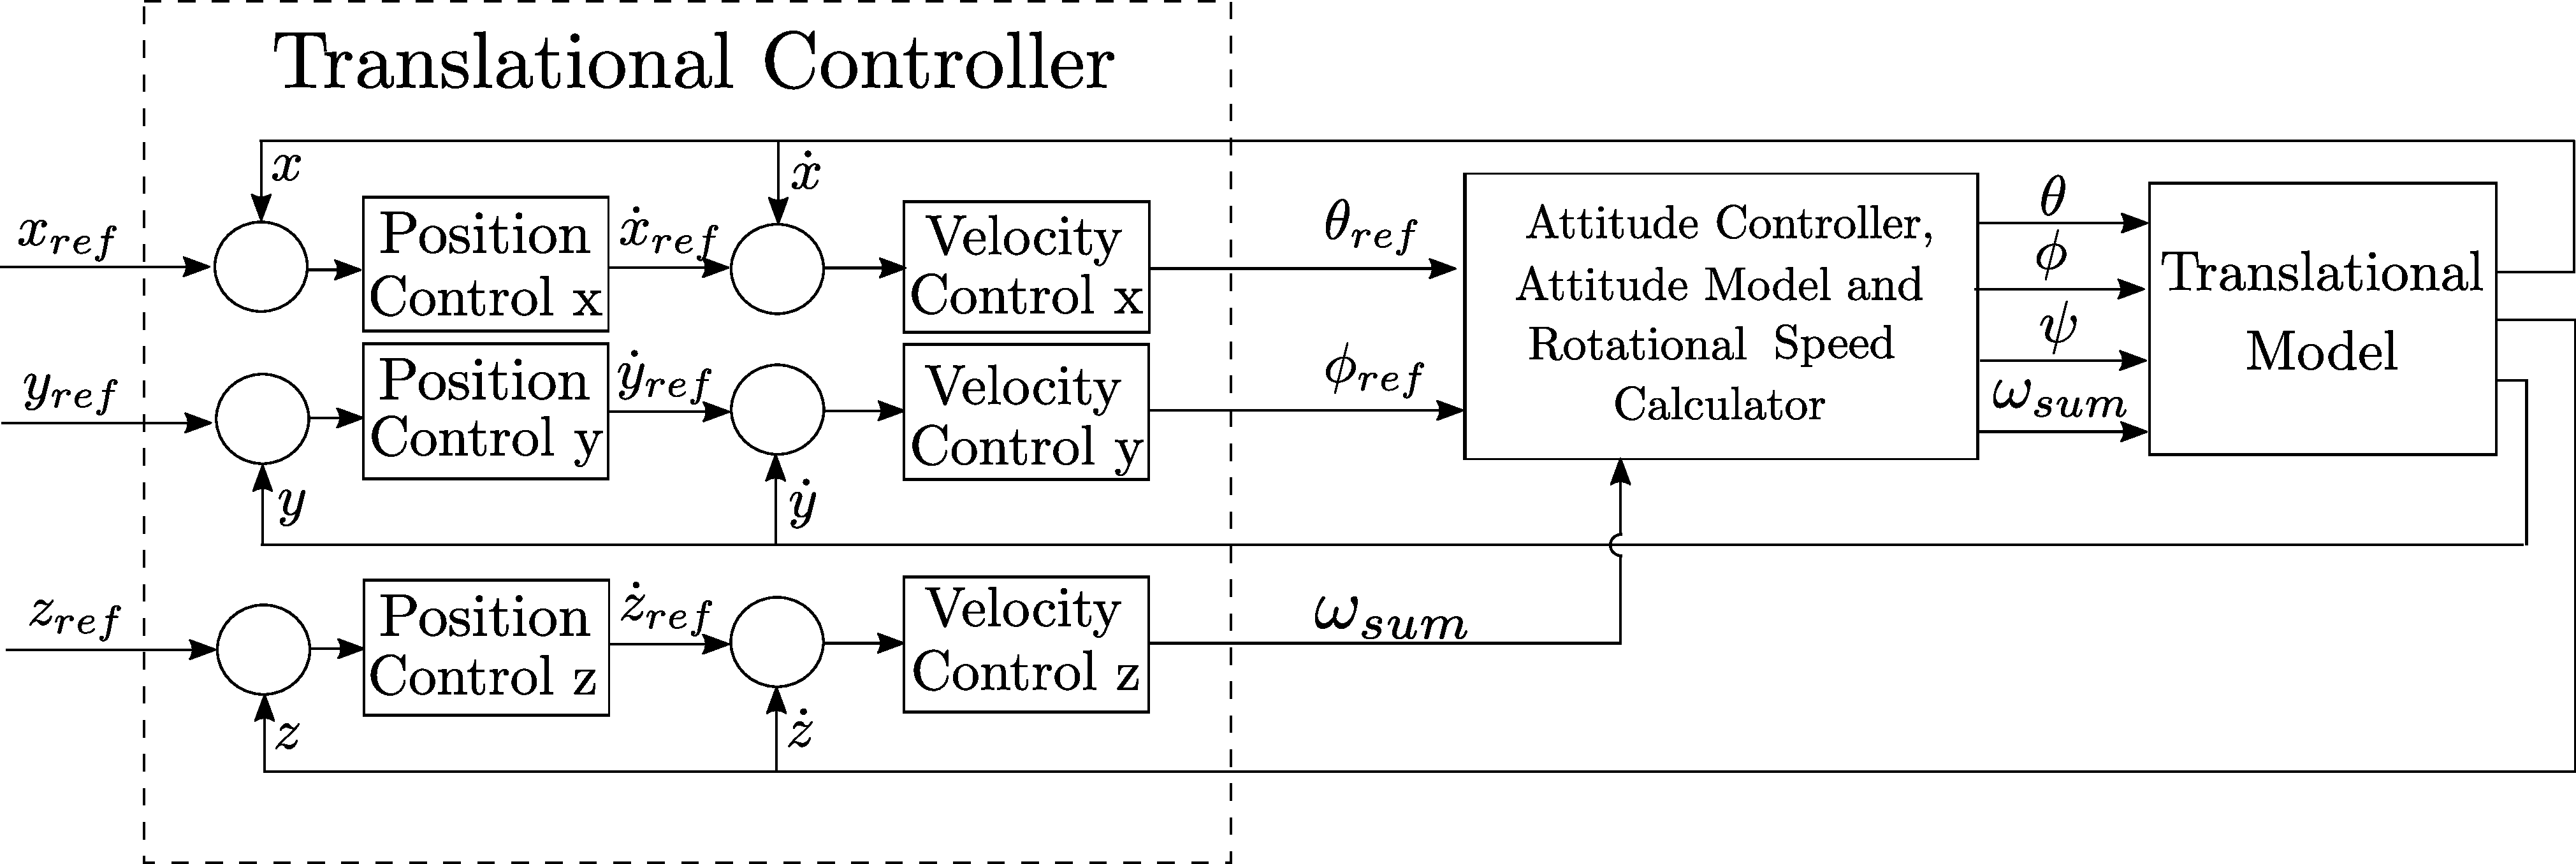
\includegraphics[scale=0.25]{figures/TranslationalControlDiagram}
	\caption{The overall figure from \autoref{fig:ControlHeadDiagram} rearrange to illustrate the translational controllers design structure.}
	\label{fig:TranslationalControlDiagram}
\end{figure}
%
For each axis, the velocity and position controllers form a cascade control structure, where the position controller sets the reference for the velocity controller. In the figure it is also possible to see how x and y controllers share similar properties as both have as output an angle reference for the attitude controller, namely $\theta_{ref}$ and $\phi_{ref}$ respectively. 
The z axis position and velocity controllers set the required sum of motor rotational speeds, $\omega_{sum}$, such that the vertical position is attained.

In the following sections the design for the mentioned controllers are explained.